\documentclass{article}
\linespread{1.3}
\usepackage[margin=50pt]{geometry}
\usepackage{amsmath, amsthm, amssymb, amsthm, tikz, fancyhdr, float, graphicx, spverbatim, systeme}
\pagestyle{fancy}
\renewcommand{\headrulewidth}{0pt}
\newcommand{\changefont}{\fontsize{15}{15}\selectfont}

\fancypagestyle{firstpageheader}{
  \fancyhead[R]{
    \changefont
    \parbox[t]{4cm}{ % Adjust width as needed
      Michael Huang\\
      EN.555.644.81\\
      Homework 1
    }
  }
}

\begin{document}

\thispagestyle{firstpageheader}
{\Large 

\section*{1.17}

A company knows that it is due to receive a certain amount of a foreign currency in four months. What type of option contract is appropriate for hedging? \\ \\ 
The risk that the company would want to hedge against would be that the exchange rate of the foreign currency would weaken against the native currency. The company would therefore want to ensure that it could lock in some of the value from the current exchange rate should that happen. By \textbf{buying a put option} on the foreign exchange rate, the company can still negate some of the downside risk.

}
{\Large 

\section*{1.18}

A US company expects to have to pay 1 million Canadian dollars in six months. Explain how the exchange rate risk can be hedged using (a) a forward contract and (b) an option.

\subsection*{(a)}

The exchange rate risk would be that the 1 million Canadian dollars appreciates against the US dollar within the next six months. The company therefore wants to try and lock in the current exchange rate to hedge against this. By using a long forward contract to lock in the current exchange rate on the same amount of Canadian dollars, the company will still pay the Canadian dollars at the current exchange rate if the exchange rate depreciates, saving money.The company should therefore enter a long forward contract to buy 1 million Canadian dollars in six months.

\subsection*{(b)}

Using options, the company could buy a call option on the same amount of Canadian dollars in six months at a fixed exchange rate. By doing so, the company can act appropriately in both scenarios: \\
- If the exchange rate appreciates, exercise the option to pay at that fixed rate rather than the more expensive rate \\
- If the exchange rate depreciates, simply let the option expire and pay the new lower rate

}
{\Large 

\section*{1.22}

Describe the profit from the following portfolio: a long forward contract on an asset and a long European put option on the asset with the same maturity as the forward contract and a strike price that is equal to the forward price of the asset at the time the portfolio is set up. \\ \\
Put simply, the portfolio includes a long forward and a long put option. Both have the same maturity and the strike price and forward price are the same. Let \(S_T\) be the price of the underlying asset at maturity, and \(K\) be the strike price / forward price. We can therefore write the payoffs at maturity as follows: \\
- Long forward: \(S_T - K\) \\ 
- Long put option: \(\max(K - S_T, 0)\) \\
So the only variable part of this is the put option. Let's break it down case by case: \\
- \(S_T \geq K\), i.e. put is out of the money and expires with value 0. The total profit would therefore be 
\[
  (S_T - K) + 0 = S_T - K
\]
- \(S_T < K\), i.e. put is in the money. The total profit would therefore be 
\[
  (S_T - K) + (K - S_T) = S_T - S_T - K + K = 0
\] 
The portfolio's overall profit is therefore just \(\max(S_T - K, 0)\). 

}
{\Large 

\section*{1.23}

In the 1980s, Bankers Trust developed index currency option notes (ICONs). These are bonds in which the amount received by the holder at maturity varies with a foreign exchange rate. One example was its trade with the Long Term Credit Bank of Japan. The ICON specified that if the yen-U.S. dollar exchange rate, \(S_T\), is greater than 169 yen per dollar at maturity (in 1995), the holder of the bond receives \$1,000. If it is less than 169 yen per dollar, the amount received by the holder of the bond is
\[
  1,000 - \max(0, 1000(\frac{169}{S_T} - 1))
\]
When the exchange rate is below 84.5, nothing is received by the holder at maturity. Show that this ICON is a combination of a regular bond and two options. \\ \\
Let's first map the payoffs at different yen-U.S. dollar exchange rates: \\
\begin{equation*}
  \begin{cases}
    \text{1,000} & S_T > 169 \\
    \text{1,000 - 1,000}(\frac{169}{S_T} - 1) = \text{2,000} - \frac{\text{169,000}}{S_T} & 84.5 \leq S_T \leq 169 \\
    0 & S_T < 84.5
  \end{cases}  
\end{equation*}
We aim to find the components of the ICON. We are given that one of the components is a regular bond, which we can easily see to be just the \$1,000 straight up. So let's rewrite the cases minus this bond component:
\begin{equation*}
  \begin{cases}
    \text{1,000 - 1,000} & S_T > 169 \\
    \text{1,000 - } (\text{2,000} - \frac{\text{169,000}}{S_T}) & 84.5 \leq S_T \leq 169 \\
    \text{1,000 - 0} & S_T < 84.5
  \end{cases}  
\end{equation*}
\begin{equation*}
  \begin{cases}
    0 & S_T > 169 \\
    \frac{\text{169,000}}{S_T} - \text{1,000} & 84.5 \leq S_T \leq 169 \\
    \text{1,000} & S_T < 84.5
  \end{cases}  
\end{equation*}
We know the remaining pieces are options. Looking at the middle component for clues, we understand that we have the inverse rate, which indicates an option on the USD portion of the exchange rate. We are generally looking for a term that fits the \(x \cdot \max(\frac{1}{S_T} - \frac{1}{K})\) form, where \(K\) is the strike price and \(x\) is some arbitrary constant. Using this form, we can rewrite the middle component as 
\[
  \frac{\text{169,000}}{S_T} - \text{1,000}
\]
\[
  = \text{169,000}(\frac{1}{S_T} - \frac{1}{169})
\]
which fits exactly the form we are looking for. We therefore have \(K = 169\) and \(x = 169,000\), which indicates that this is some call option to buy 169,000 yen with strike price of 169. We know that we lose money as the price falls, which indicates that we are short this option, as we lose money as yen the yen strengthens (lowering in \(K\)). \\
Finally, we need to find another option component which handles the payoff when the rate goes below 84.5. The first option gives us a big hint -- we need to have a long position on some call with strike price 84.5. Intuitively, we try for a term in the form of \(\text{169,000}(\frac{1}{S_T} - \frac{1}{84.5})\) which represents this call option. We know that the ICON pays 0 when \(S_T < 84.5\). It needs to become positive and cancel out the middle option's losses as we dip below 84.5. We can test this to confirm the intuition, for example at \(S_T = 50\), the payoff is 
\[
  \text{1,000} - \text{169,000}(\frac{1}{S_T} - \frac{1}{169}) + \text{169,000}(\frac{1}{S_T} - \frac{1}{84.5})
\]
\[
  = \text{1,000} - \text{169,000}(\frac{1}{50} - \frac{1}{169}) + \text{169,000}(\frac{1}{50} - \frac{1}{84.5})
\]
\[
  = \text{1,000} - \text{169,000}(0.01408284023) + \text{169,000}(0.00816568047)
\]
\[
  = \text{1,000} - \text{2,380} + \text{1,380}
\]
\[
  = 0 
\]
as we expected.
\\ \\ 
\textbf{We therefore can represent the ICON as the following: \\
- A regular \$1,000 bond \\
- A short position in a call option to buy 169,000 yen with strike price \(\frac{1}{169}\) \\
- A long position in a call option to buy 169,000 yen with strike price \(\frac{1}{84.5}\)
}

}
{\Large 

\section*{1.39}

Suppose that in the situation of Table 1.1 a corporate treasurer said: “I will have £1 million to sell in six months. If the exchange rate is less than 1.52, I want you to give me 1.52. If it is greater than 1.58 I will accept 1.58. If the exchange rate is between 1.52 and 1.58, I will sell the sterling for the exchange rate.” How could you use options to satisfy the treasurer?
\begin{figure}[h!]
  \centering
  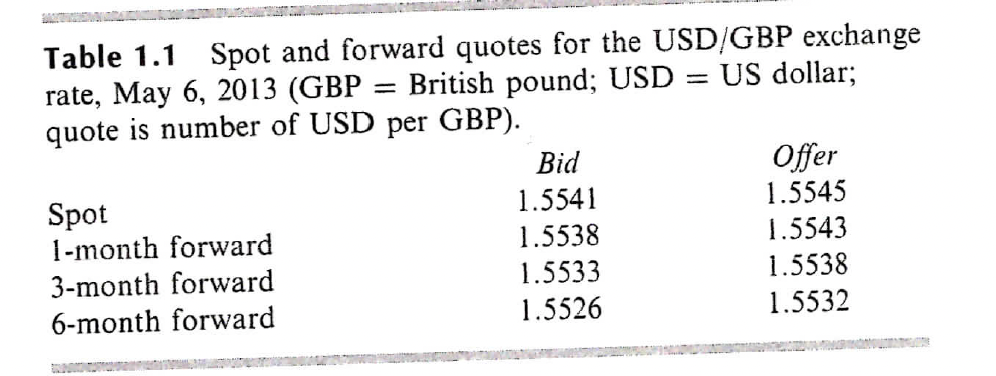
\includegraphics[width=400pt]{Table 1.1.png}
\end{figure} \\ 
The corporate treasurer is essentially saying that they have a floor at 1.52 and a cap at 1.58, i.e. they have a guaranteed minimum sale price at 1.52 and will give up upside above 1.58 to maximize their sale price at 1.58. Breaking each of these down by definition: \\
- Guaranteed minimum sale price at 1.52: The corporate treasurer should buy a put option at strike price of 1.52 for £1 million in six months. This works since should the exchange rate go below 1.52, the corporate treasurer can then sell the £1 million at 1.52 as they said, and let the option expire otherwise. \\
- Maximum sale price at 1.58: The corporate treasurer should sell a call option with a strike price of 1.58 for £1 million in six months. This works since if the exchange rate goes above 1.58, the buyer would exercise the option against the corporate treasurer and get the £1 million at 1.58. Otherwise, the option can expire and the sale can proceed accordingly. \\
Using both of these options, the corporate treasurer's terms should be satisfied, with anything between the two rates leading to both options expiring and the corporate treasurer just selling at the spot rate. 

}
{\Large 

\section*{1.40}

Describe how foreign currency options can be used for hedging in the situation considered in Section 1.7 so that (a) ImportCo is guaranteed that its exchange rate will be less than 1.5700, and (b) ExportCo is guaranteed that its exchange rate will be at least 1.5300. Use DerivaGem to calculate the cost of setting up the hedge in each case assuming that the exchange rate volatility is 12\%, interest rates in the United States are 5\% and interest rates in Britain are 5.7\%. Assume that the current exchange rate is the average of the bid and offer in Table 1.1. 
\begin{figure}[h!]
  \centering
  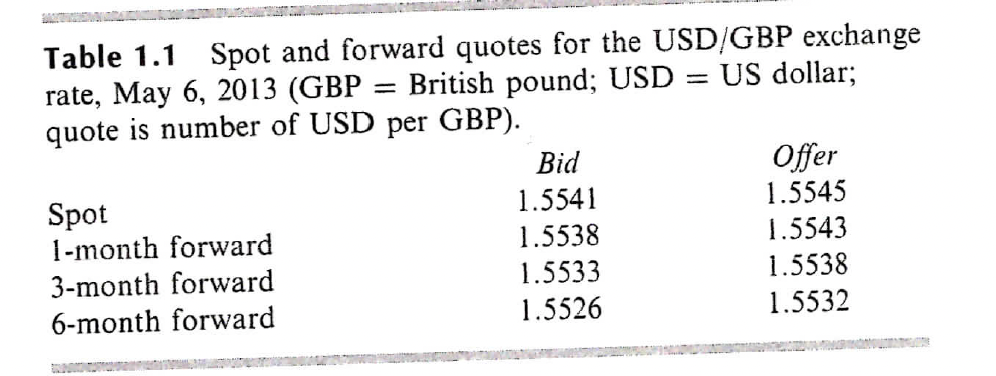
\includegraphics[width=400pt]{Table 1.1.png}
\end{figure} \\

The current exchange rate is the average of the spot bid and offer, so it is simply \(\frac{1.5541 + 1.5545}{2} = 1.5543\). I also set the Option Type to "Binomial: European" as we don't exercise before expiry in this case. 

\subsection*{(a)}

ImportCo needs to guarantee that its exchange rate will be less than 1.5700. ImportCo needs the ability to buy GBP at the same 10 million pound notional with strike of 1.5700 to guarantee that the exchange rate will cap at 1.5700. This describes buying a call option so that ImportCo will always buy the pounds at 1.5700 or lower. 
\begin{figure}[h!]
  \centering
  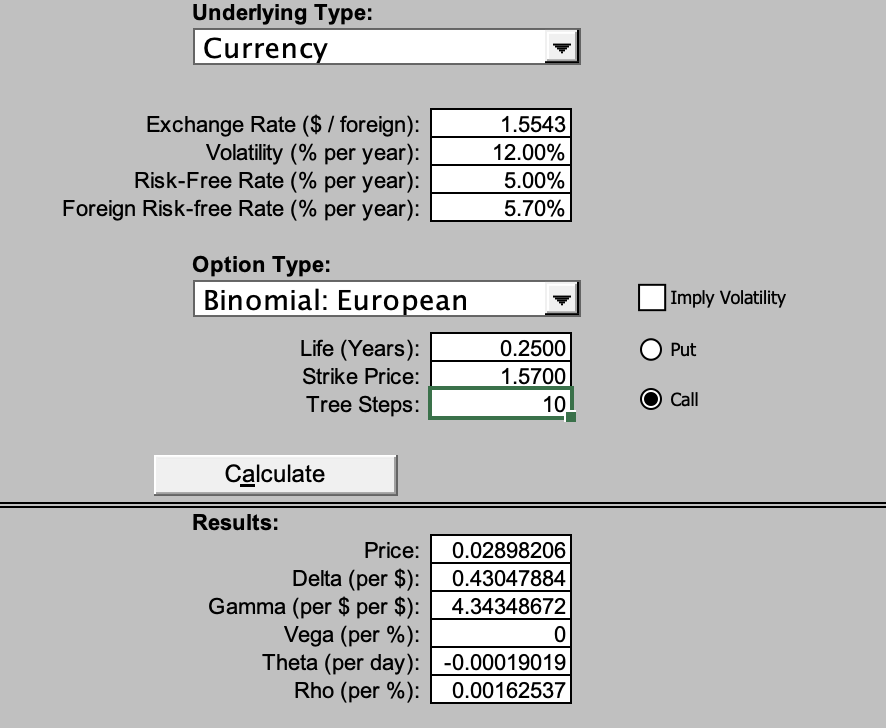
\includegraphics[width=400pt]{1_40_a_derivagem.png}
\end{figure} \\ \\ \\ \\ 
Looking at DerivaGem, we see that the price is about \$0.02898206, which indicates that the cost is about \textbf{\$289,820.60} for 10 million GBP. 

\subsection*{(b)}

ExportCo needs to guarantee that its exchange rate will be at least 1.5300. ExportCo needs to sell GBP at the same 30 million pound notional at strike of 1.53000. This describes buying a put option so that ExportCo will always sell the pounds at 1.5300 or higher. 
\begin{figure}[h!]
  \centering
  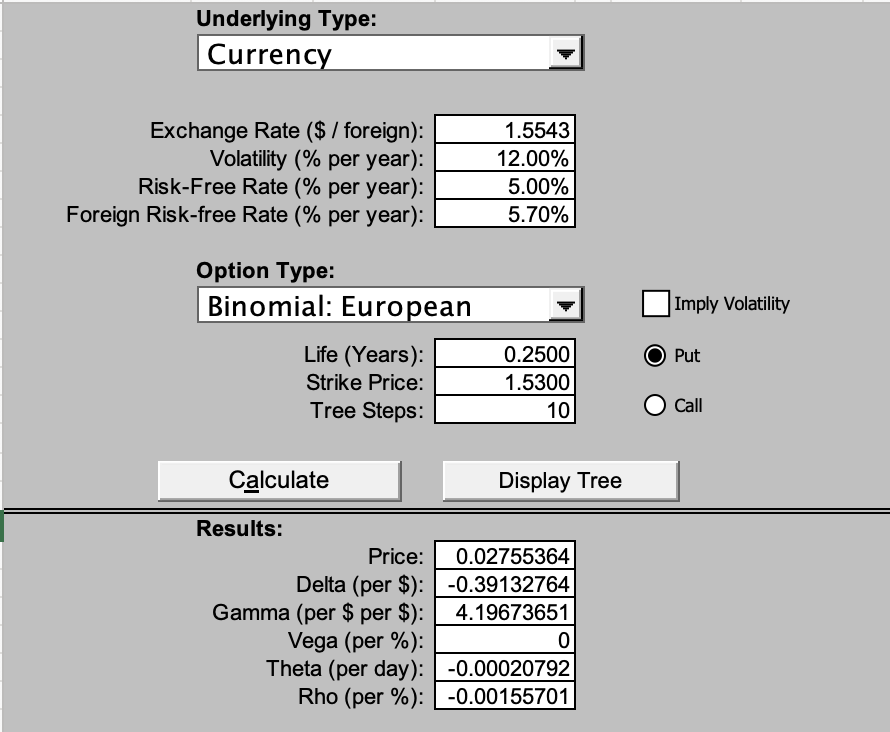
\includegraphics[width=400pt]{1_40_b_derivagem.png}
\end{figure} \\ \\ \\ \\ \\ \\ \\ \\
Looking at DerivaGem, we see that the price is about \$0.02755364, which indicates that the cost is about \textbf{\$826,609.20} for 30 million GBP.

}
{\Large 

\section*{2.15}

At the end of one day a clearing house member is long 100 contracts, and the settlement price is \$50,000 per contract. The original margin is \$2,000 per contract. On the following day the member becomes responsible for clearing an additional 20 long contracts, entered into at a price of \$51,000 per contract. The settlement price at the end of this day is \$50,200. How much does the member have to add to its margin account with the exchange clearing house? \\ \\
The initial margin for the additional 20 long contracts would be \(20 \cdot \) \$2,000 = \$40,000 needing to be initially deposited. \\
The existing contracts gain \((\text{\$50,200} - \text{\$50,000}) \cdot 100 = \text{\$200} \cdot 100 = \text{\$20,000}\) credited. \\
The new contracts lose \((\text{\$51,000} - \text{\$50,200}) \cdot 20 = \text{\$800} \cdot 20 = \text{\$16,000}\) as loss. \\ 
We are therefore left with \(\text{\$40,000} - \text{\$20,000} + \text{\$16,000} = \textbf{\$36,000} \) needing to be added to the margin account by the clearing house member.

}
{\Large 

\section*{2.21}

What do you think would happen if an exchange started trading a contract in which the quality of the underlying asset was incompletely specified? \\ \\
If an exchange started trading a contract in which the quality of the underlying asset was incompletely specified, then the party with the short position gets to choose, so the short side would likely deliver the worst quality asset possible. In turn, the long side would adapt and the corresponding contracts would then be priced according to the lowest quality asset. This would lead to overall uncertainty in the market and less liquidity as a result of the uncertainty or pessimism around the asset quality.

}
{\Large 

\section*{2.22}

“When a futures contract is traded on the floor of the exchange, it may be the case that the open interest increases by one, stays the same, or decreases by one.” Explain this statement. \\ \\ 
Let's explain the statement by walking through the different cases of opening or closing out positions on both the buyer and seller side: \\
- Buyer opens, seller opens: The open interest increases by one \\
- Buyer opens, seller closes; buyer closes, seller opens: The open interest stays the same, as the positions being opened and closed is offset \\
- Buyer closes, seller closes: The open interest decreases by one \\ 
Which accounts for all situations mentioned in the statement. 

}
{\Large 

\section*{2.28}

Explain what is meant by open interest. Why does the open interest usually decline during the month preceding the delivery month? On a particular day, there were 2,000 trades in a particular futures contract. This means that there were 2000 buyers (going long) and 2000 sellers (going short). Of the 2,000 buyers, 1,400 were closing out positions and 600 were entering into new positions. Of the 2,000 sellers, 1,200 were closing out positions and 800 were entering into new positions. What is the impact of the day's trading on open interest? \\ \\
Open interest, which indicates the number of outstanding contracts, usually declines during the month preceding the delivery month since traders will tend to close out their positions before actual delivery happens. \\ \\
We are given that 600 buyers are entering new positions, which means that there are 600 longs created. We are also given that 1,200 sellers closing out positions, which means that there are 1,200 longs closed out. The net open interest is therefore 600 - 1,200 = -600, which means that \textbf{open interest decreased by 600}.

}
{\Large 

\section*{2.31}

Suppose that there are no storage costs for crude oil and the interest rate for borrowing or lending is 5\% per annum. How could you make money if the June and December futures contracts for a particular year trade at \$80 and \$86? \\ \\
Given that the June oil contract is at \$80, and the interest rate is at 5\% per annum, we can find the interest rate for getting the June contract and taking delivery would be \(\$80 \cdot 0.05 \cdot \frac{1}{2} = \$2\) per unit. Therefore, the total cost including the loaned amount for buying the June contract would \$80 + \$2 = \$82. This is less than the \$86 at which the December futures contracts are trading at. We could therefore make profit by entering into long June futures contracts and subsequently entering into short December future contracts. So we would buy contracts, take delivery in June, then sell and Deliver in December and make a profit. 

}

\end{document}